\chapter{Appendix}
\subsection*{Shouldice Limburg Simulation Dashboard}
\begin{figure}[htpb]
	\centering
	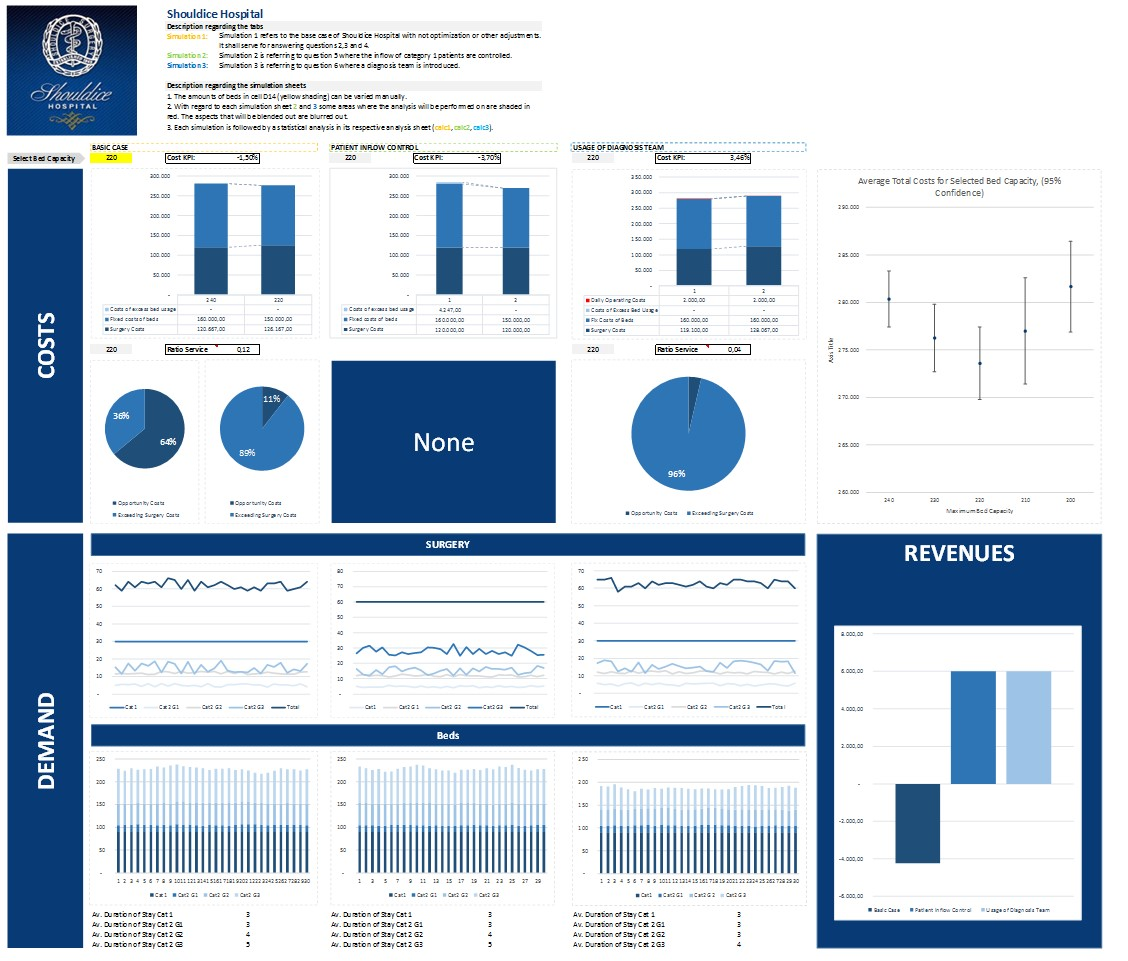
\includegraphics[width=\textwidth]{Picture5.JPG}
	\label{Dashboard}
\end{figure}
\newpage
\subsection*{Simulation for Basic Case}\label{sim1}
\begin{figure}[htpb]
	\centering
	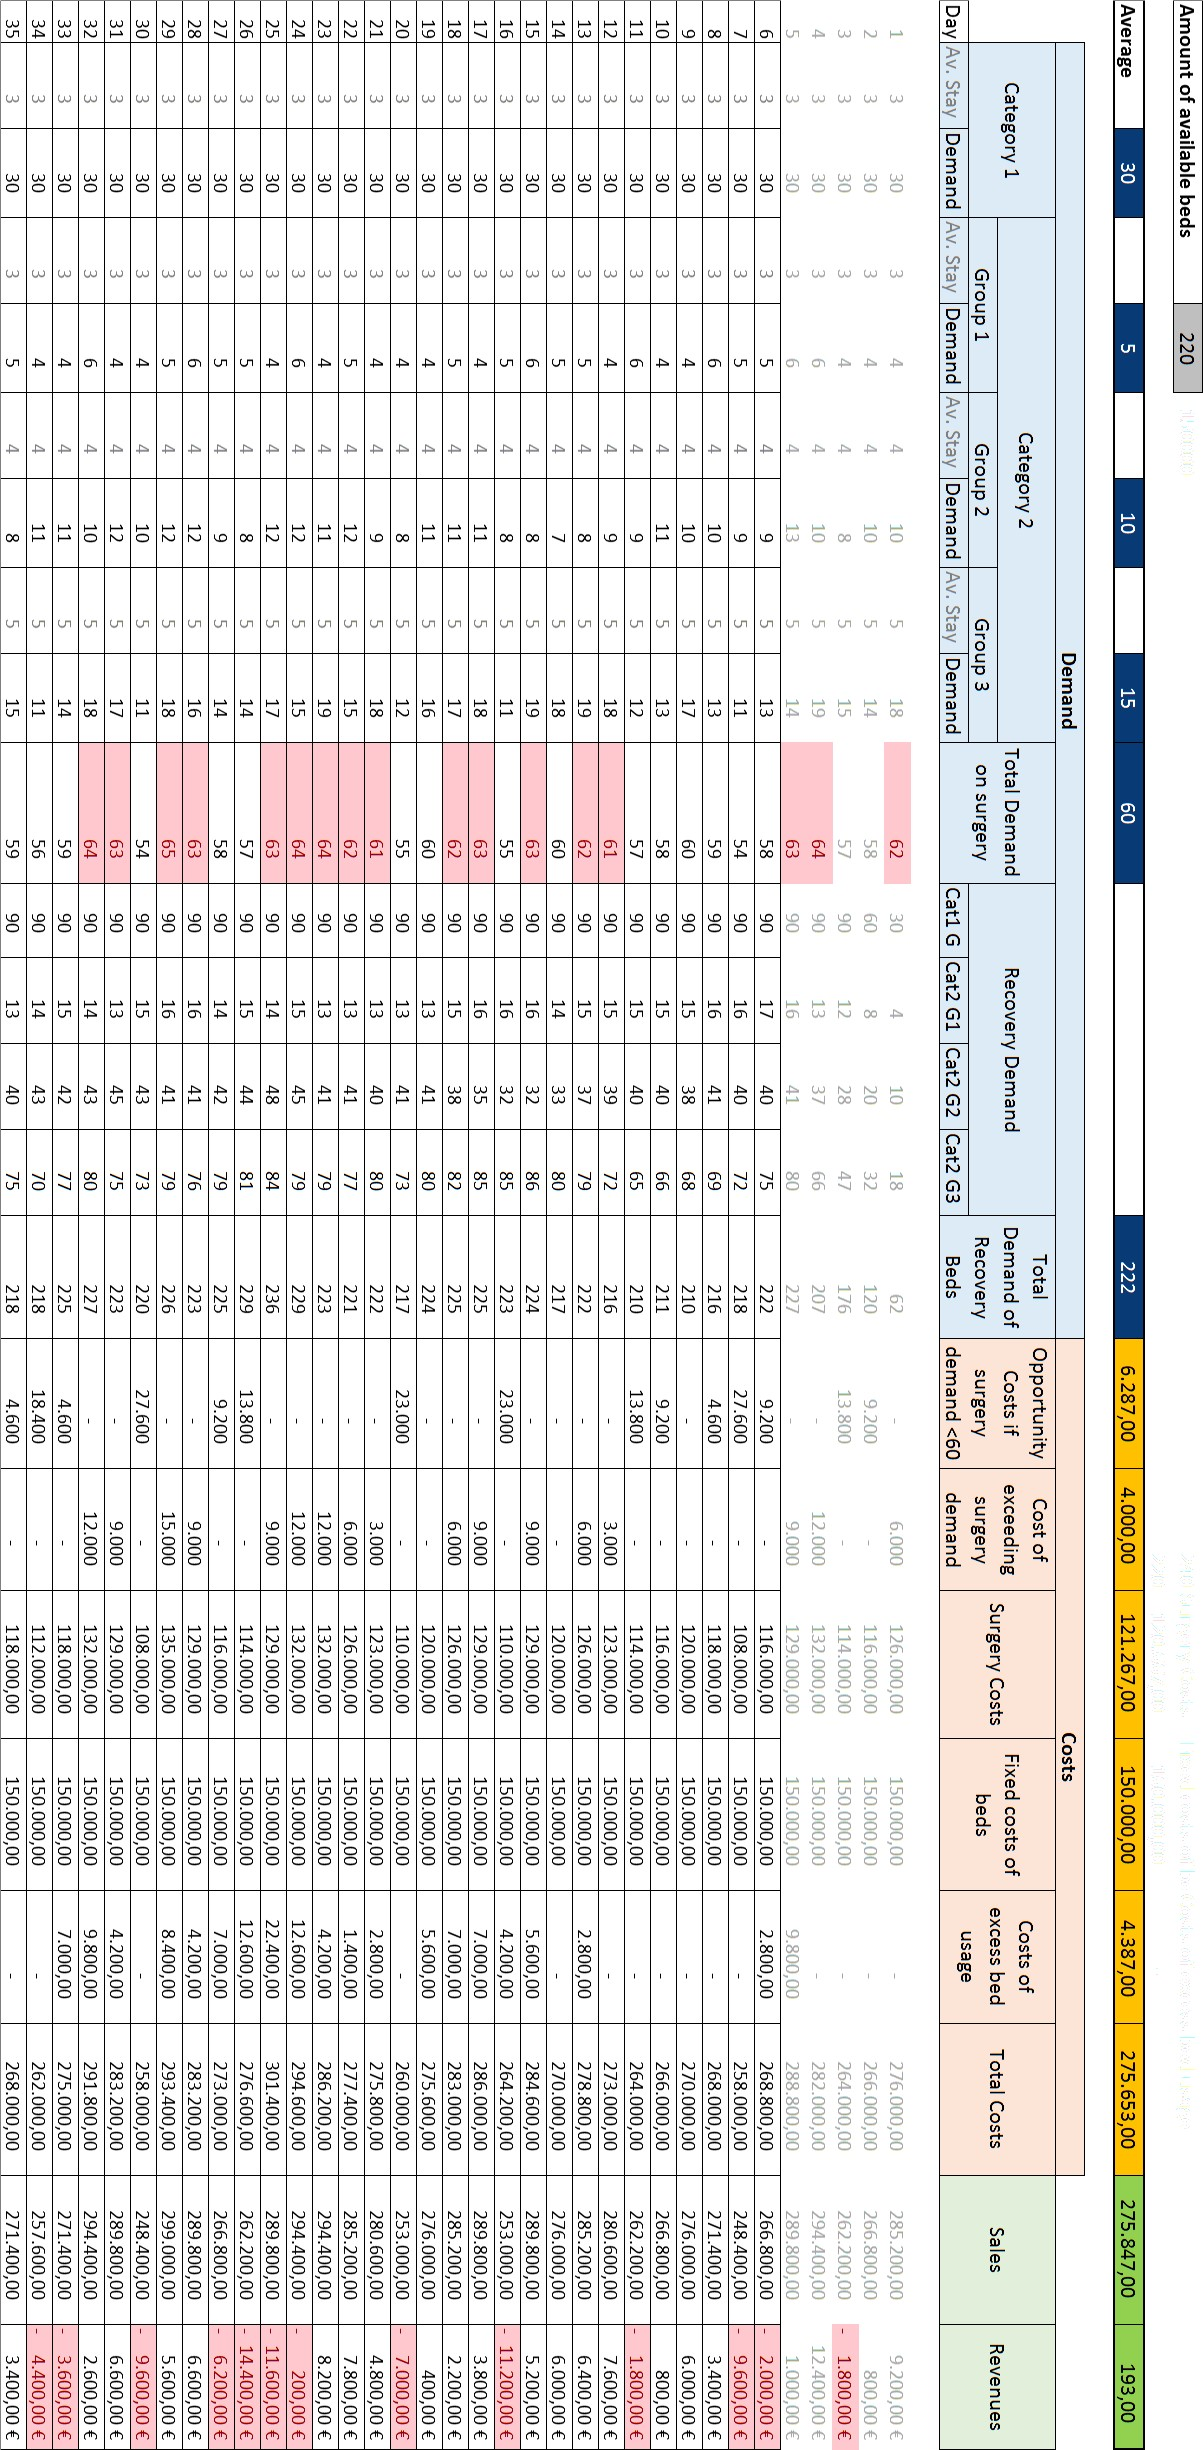
\includegraphics[width=0.53\textwidth]{Picture12.JPG}
\end{figure}
\newpage
\subsection*{Simulation for Patient Inflow Control}
\begin{figure}[htpb]
	\centering
	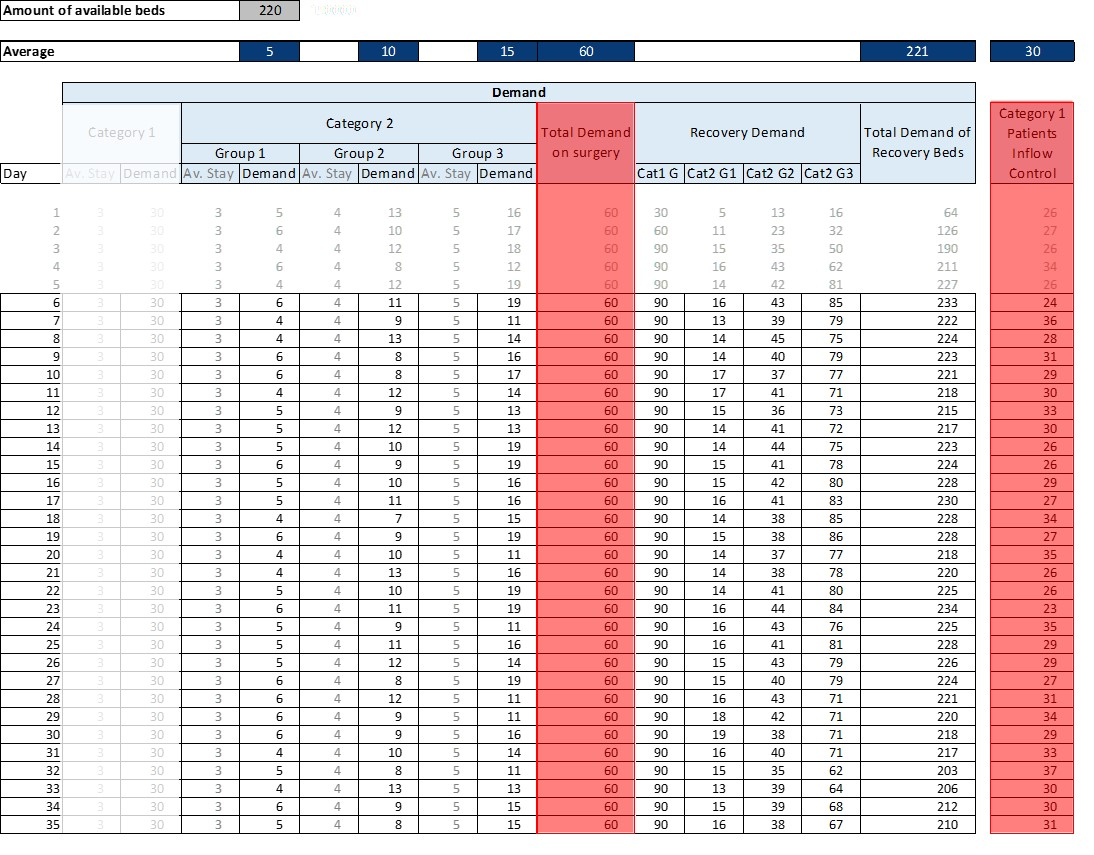
\includegraphics[width=\textwidth]{Picture13.JPG}
	\label{sim2}
\end{figure}
\newpage
\subsection*{Simulation for Implementation of Diagnosis Team}
\begin{figure}[htpb]
	\centering
	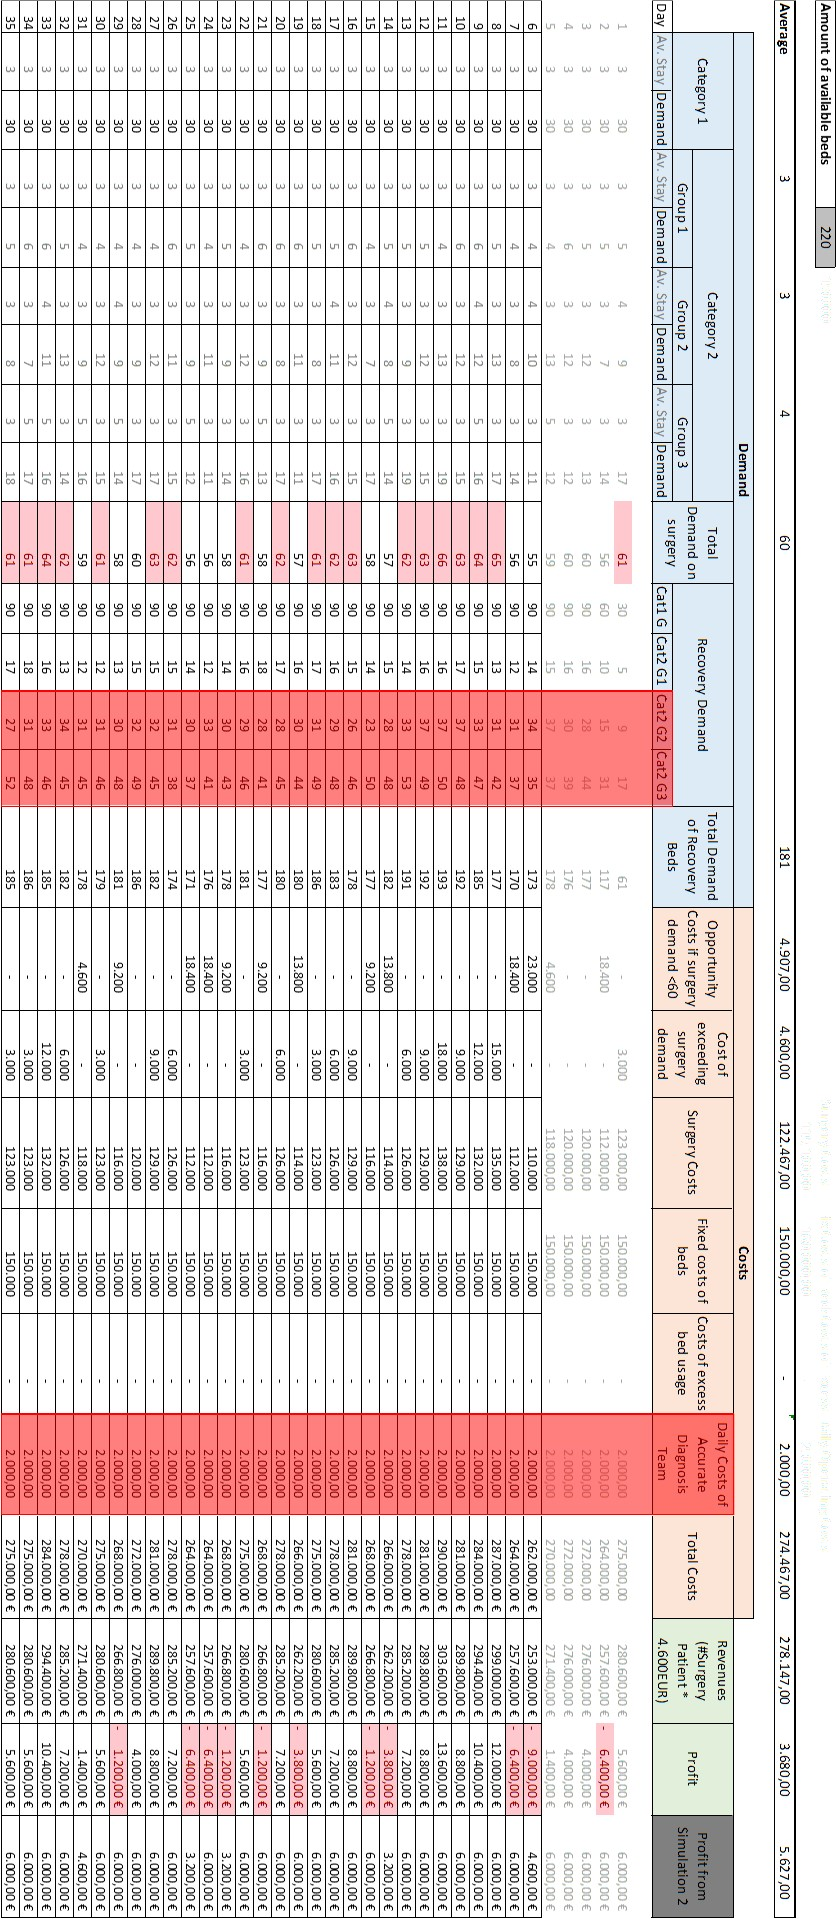
\includegraphics[width=0.45\textwidth]{Picture14.JPG}
	\label{sim3}
\end{figure}
\newpage
\subsection*{Technical Explanation Regarding Simulation}
For the analysis at hand three different situations based from the status quo have been modelled and simulated using Microsoft Excel and the UMS Tool macro add-in. The basic case in Excel of the simulation is depicted in "Simulation 1". 

In order to generate random values for the unknown variables regarding category 2 patients which are uniformly distributed we have used a "drawuniform" formula. To make sure that the all values are equally distributed the lower value of the uniform range had to be deducted by 0,5 and the higher value of the uniform range had to be increased by 0,5. The maximum bed capacity was deducted stepwise by 10 beds and each state of total cost resulting from this was analyzed using the data analysis function from excel in order to evaluate the 95\% confidence.

The case of patient inflow controlls is depicted in "Simulation 2". Here the total surgery patients column was fixed with 60 patients per day and the patient inflow from category 1 patient was made flexible. The specific changes with regard to simulation 1 are highlighted in red shading in the Excel sheet.

The case of the implementation of a diagnosis team is depicted in "Simulation 3". For patients from category 2, sub-groups 2 and 3, the average duration of stay could be influenced by using a diagnosis team. The probability of correct diagnosis was given by 80\% and 20\% probability for a wrong diagnosis. This represents a binomial distribution. In order to model this in Excel the "drawdiscrete" formula was used. The specific columns which were adjusted with respect to simulation 2 are shaded in red in the Excel sheet.

Simulation via the UMS Tool were runned with 1.000 replications. According to \cite[p.501 f.]{ragsdale} 300 replications represent a sufficient number of replications. Because of sufficient computing power we decided to run 1.000 replications then.